\documentclass[a4paper,14pt]{article}

\usepackage{comment} % Para comentar várias linhas ao mesmo tempo

%matemática
\usepackage{amsmath}
\usepackage{amssymb}

%diagramação
\usepackage{extsizes}
\everymath{\displaystyle}
\usepackage{geometry}
\usepackage{fancyhdr}
\usepackage{multicol}
\usepackage{graphicx}
\usepackage[brazil]{babel}
\usepackage[shortlabels]{enumitem}
\usepackage{cancel}
\usepackage{textcomp}
\usepackage{tcolorbox}

%tabelas
\usepackage{array} % Para melhor formatação de tabelas
\usepackage{longtable}
\usepackage{booktabs}  % Para linhas horizontais mais bonitas
\usepackage{float}   % Para usar o modificador [H]
\usepackage{caption} % Para usar legendas em tabelas
\usepackage{wrapfig} % Para usar tabelas e figuras flutuantes

\begin{comment}
%tikzpicture
\usepackage{tikz}
\usepackage{scalerel}
\usepackage{pict2e}
\usepackage{tkz-euclide}
\usetikzlibrary{calc}
\usetikzlibrary{patterns,arrows.meta}
\usetikzlibrary{shadows}
\usetikzlibrary{external}
\end{comment}
	
%pgfplots
\usepackage{pgfplots}
\pgfplotsset{compat=newest}
\usepgfplotslibrary{statistics}
\usepgfplotslibrary{fillbetween}

%colours
\usepackage{xcolor}



\columnsep=2cm
\hoffset=0cm
\textwidth=8cm
\setlength{\columnseprule}{.1pt}
\setlength{\columnsep}{2cm}
\renewcommand{\headrulewidth}{0pt}
\geometry{top=1in, bottom=1in, left=0.7in, right=0.5in}

\pagestyle{fancy}
\fancyhf{}
\fancyfoot[C]{\thepage}

\begin{document}
	
	\noindent\textbf{6FMA74 - Matemática} 
	
	\begin{center}Exercícios de conjuntos com informações quantitativas (Versão estudante)
	\end{center}
	
	\noindent\textbf{Nome:} \underline{\hspace{10cm}}
	\noindent\textbf{Data:} \underline{\hspace{4cm}}
	
	%\section*{Questões de Matemática}
	
	\begin{multicols}{2}
    	\begin{enumerate}
   			\item João tem em sua carteira uma nota de dois reais, uma nota de cinco reais, uma nota de dez reais, uma nota de vinte reais e uma nota de cinquenta reais. \\
   			Se um amigo lhe pedir dinheiro emprestado, de quantas maneiras distintas João poderá ajudá-lo? \\\\\\\\\\\\\\\\\\\\\\\\\\\\\\\\\\\\\\\\\\\\\\\\\\\\\\
   			\item Em um aplicativo de música, Pedro montou um álbum no qual é possível escolher quais músicas ele vai ouvir de 512 maneiras diferentes (desde nenhuma música até todas elas). Quantas músicas tem o álbum que Pedro montou? \newpage
   			\item Acrescentando três novos livros à minha coleção, verifiquei que o número de maneiras que posso escolher livros para colocar em uma estante aumentou de 112. Quantos livros eu possuia originalmente? \\\\\\\\\\\\\\\\\\\\\\\\\\\\\\\\\\\\\\\\\\\\\\\\\\\\\\\\\\\\\\\\\\\\\\
   			\textbf{Desafio olímpico} \\\\
   			Em um jogo de tabuleiro, representado na figura abaixo, os irmãos Daniel e Cláudio utilizam um peão para caminhar de uma casa a outra. A regra do jogo permite que o peão caminhe nas linhas em direção a qualquer casa, com exceção da casa D, que finaliza o jogo. De quantas maneiras Cláudio poderá mover seu peão de A até D com exatamente 15 movimentos? 
   			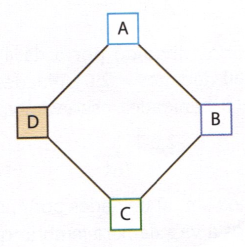
\includegraphics[width=1\linewidth]{6FMA74_imagens/imagem1}
   			%9 e 10
   			\begin{enumerate}[a)]
   				\item 1 024
   				\item 256
   				\item 128
   				\item 32
   				\item 16 \newpage
   			\end{enumerate} 
   			\item Flávia tem uma pulseira com contas que podem ser retiradas. Cada conta tem uma cor diferente: amarela, azul, cinza, preta, rosa, roxa, verde e vermelha. Se não importa a ordem das contas na pulseira, de quantas maneiras diferentes é possível montá-la (desde nenhuma conta até todas elas)? \\\\\\\\\\\\\\\\\\\\\\\\\\\\\\\\\\\\\\\\\\\\\\\\\\\\\\\\\\\\\\
   			\item A biblioteca de uma escola recebeu uma doação com 4 livros de Geometria. A bibliotecária verificou que o número de maneiras que ela pode escolher os livros para colocar na prateleira referente a Geometria aumentou de 960. Quantos livros de Geometria a biblioteca possuía antes da doação?
   		\end{enumerate}
        $~$ \\ $~$ \\ $~$ \\ $~$ \\ $~$ \\ $~$ \\ $~$ \\ $~$ \\ $~$ \\ $~$ \\ $~$ \\ $~$ \\ $~$ \\ $~$ \\ $~$ \\ $~$ \\ $~$ \\ $~$ \\ $~$ \\ $~$ \\ $~$ \\ $~$ \\ $~$ \\ $~$ \\ $~$ \\ $~$ \\ $~$ \\ $~$ \\ $~$ \\ $~$ 
        \end{multicols}
\end{document}